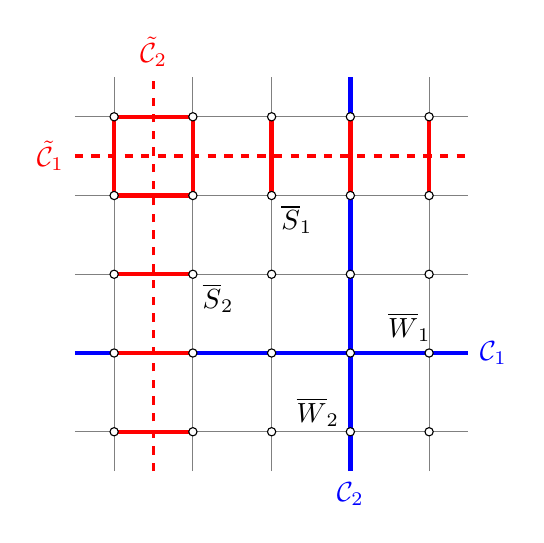
\begin{tikzpicture}[
        site/.style = {circle, inner sep=0 pt, minimum size=3pt, draw=black, fill=white},
    ]
    % lattice grid
    \draw[Gray,thin] (-0.5,-0.5) grid (4.5,4.5);

    % Wilson loops
    \draw[Blue, ultra thick]
        (-0.5, 1) -- (4.5, 1)
        node [pos=1, right] {$\mathcal{C}_1$}
        node [pos=0.85, above, black] {$\overline{W}_1$}
        ;
    \draw[Blue, ultra thick]
        (3, -0.5) -- (3, 4.5)
        node [pos=0, below] {$\mathcal{C}_2$}
        node [pos=0.15, left, black] {$\overline{W}_2$}
        ;

    % 't Hooft strings
    \draw[Red, very thick, dashed]
        (-0.5,3.5) -- (4.5,3.5)
        node[pos=0, left] {$\tilde{\mathcal{C}}_1$}
        ;
    \foreach \x in {0,...,4} { \draw[Red, ultra thick] (\x, 3) -- +(0, 1); }
    \draw (2,3) node [below right] {$\overline{S}_1$};
    \draw[Red, very thick, dashed]
        (0.5,-0.5) -- (0.5,4.5)
        node[pos=1, above] {$\tilde{\mathcal{C}}_2$}
        ;
    \foreach \y in {0,...,4} { \draw[Red, ultra thick] (0, \y) -- +(1, 0); }
    \draw (1,2) node [below right] {$\overline{S}_2$};
    \foreach \y in {0,...,4} \foreach \x in {0,...,4} \draw (\x,\y) node [site] {};
\end{tikzpicture}
